\documentclass[conference]{IEEEtran} % Usa la classe IEEEtran per formattazione simile

\usepackage{amsmath}
\usepackage{graphicx}



\begin{document}

\title{Exploring the Adversarial Robustness of AI-generated Image Detectors}

\author{
    \IEEEauthorblockN{Thomas Lazzerini, Samuele Cappelletti, Martina D'Angelo}
    \IEEEauthorblockA{
        University of Trento
    }
}

\maketitle

\begin{abstract}
    TODO
\end{abstract}

\section{Introduction}
    Synthetic images are now flooding the real world. From online dating sites to social media, fake profiles and scams are everywhere. The problem with synthetic images is that, while some of them are funny and harmless, others could be harmful, they could be exploited by malicious users \cite{carlini2020evading}. In relation to this, in the image forensic field there is a continuous fight between \textit{fake image detectors} and \textit{adversarial attacks}. On one hand, the detectors try to distinguish fake images from real ones, while, on the other hand, the attacks try to trick the detectors by manipulating the images (both real and fake ones). In order to detect fake images, we can exploit the traces/artifacts that fake image generators leave on the generated images. To do so, we have two main types of techniques: the \textit{low-level forensic techniques} and the \textit{high-level forensic techniques}. To former focuses on the pixel-level artifacts, which are almost invisible to the human eye. The latter focuses on physical inconsistencies and on repeated and uniform patterns, both of which are mostly visible to the human eye. Examples of physical inconsistencies are lighting, shadows, reflections or vanishing points inconsistencies \cite{farid2022lighting}\cite{farid2022perspective}. While, an example of repeated and uniform patterns, typical of GAN-based image generators, is the generation of the mouth, the nose and the eyes always in the same position \cite{mundra2023exposing}. In general, we prefer to rely on low-level artifacts since fake image generators are becoming smarter every day, thus they are learning to generate always more realistic images, with fewer physical inconsistencies.

\section{Detectors}

    In this section we will briefly describe a couple of fake image detectors: one uses CLIP to extract the feature vectors from the images \cite{cozzolino2024raising} and one identifies the low-level traces/artifacts by training a GAN and a Diffusion Model \cite{corvi2023detection}.

    \subsection{CLIP-Based Detector}
        Many SoTA fake image detectors works very well in detecting fake images that are generated by an image generator of the same family of the generator that generated the images that they were trained on. But, the problem is that their performance decreases a lot when trying to detect images generated by another type of detector. For example, if the images used to train the detector were generated by a GAN-based generator, then the detector is good in detecting images generated by other GAN-based generators but, it is bad in detecting images generated by a Diffusion-based generator. Moreover, the SoTA detectors hardly generalize to new and unseen generative methods.

        On the other hand, the CLIP-based detector proposed by \cite{cozzolino2024raising} works well in detecting images generated by any type of generator, both with and without augmentations (e.g., cropping, resizing, compression, etc.). Moreover, the performance of this CLIP-based method is similar to the one of the SoTA detectors in the in-distribution scenario but, it has a significant improvement in the out-of-distribution scenario. This is thanks to the fact that the CLIP features achieve an excellent generalization and robustness even with a few examples (e.g., 1k or 10k).

        The idea of this CLIP-based method is to collect N real images.
        
        FINIRE DESCRIZIONE E CONCLUSIONE DETECTOR


    %\begin{figure}[h]
    %    \centering
    %    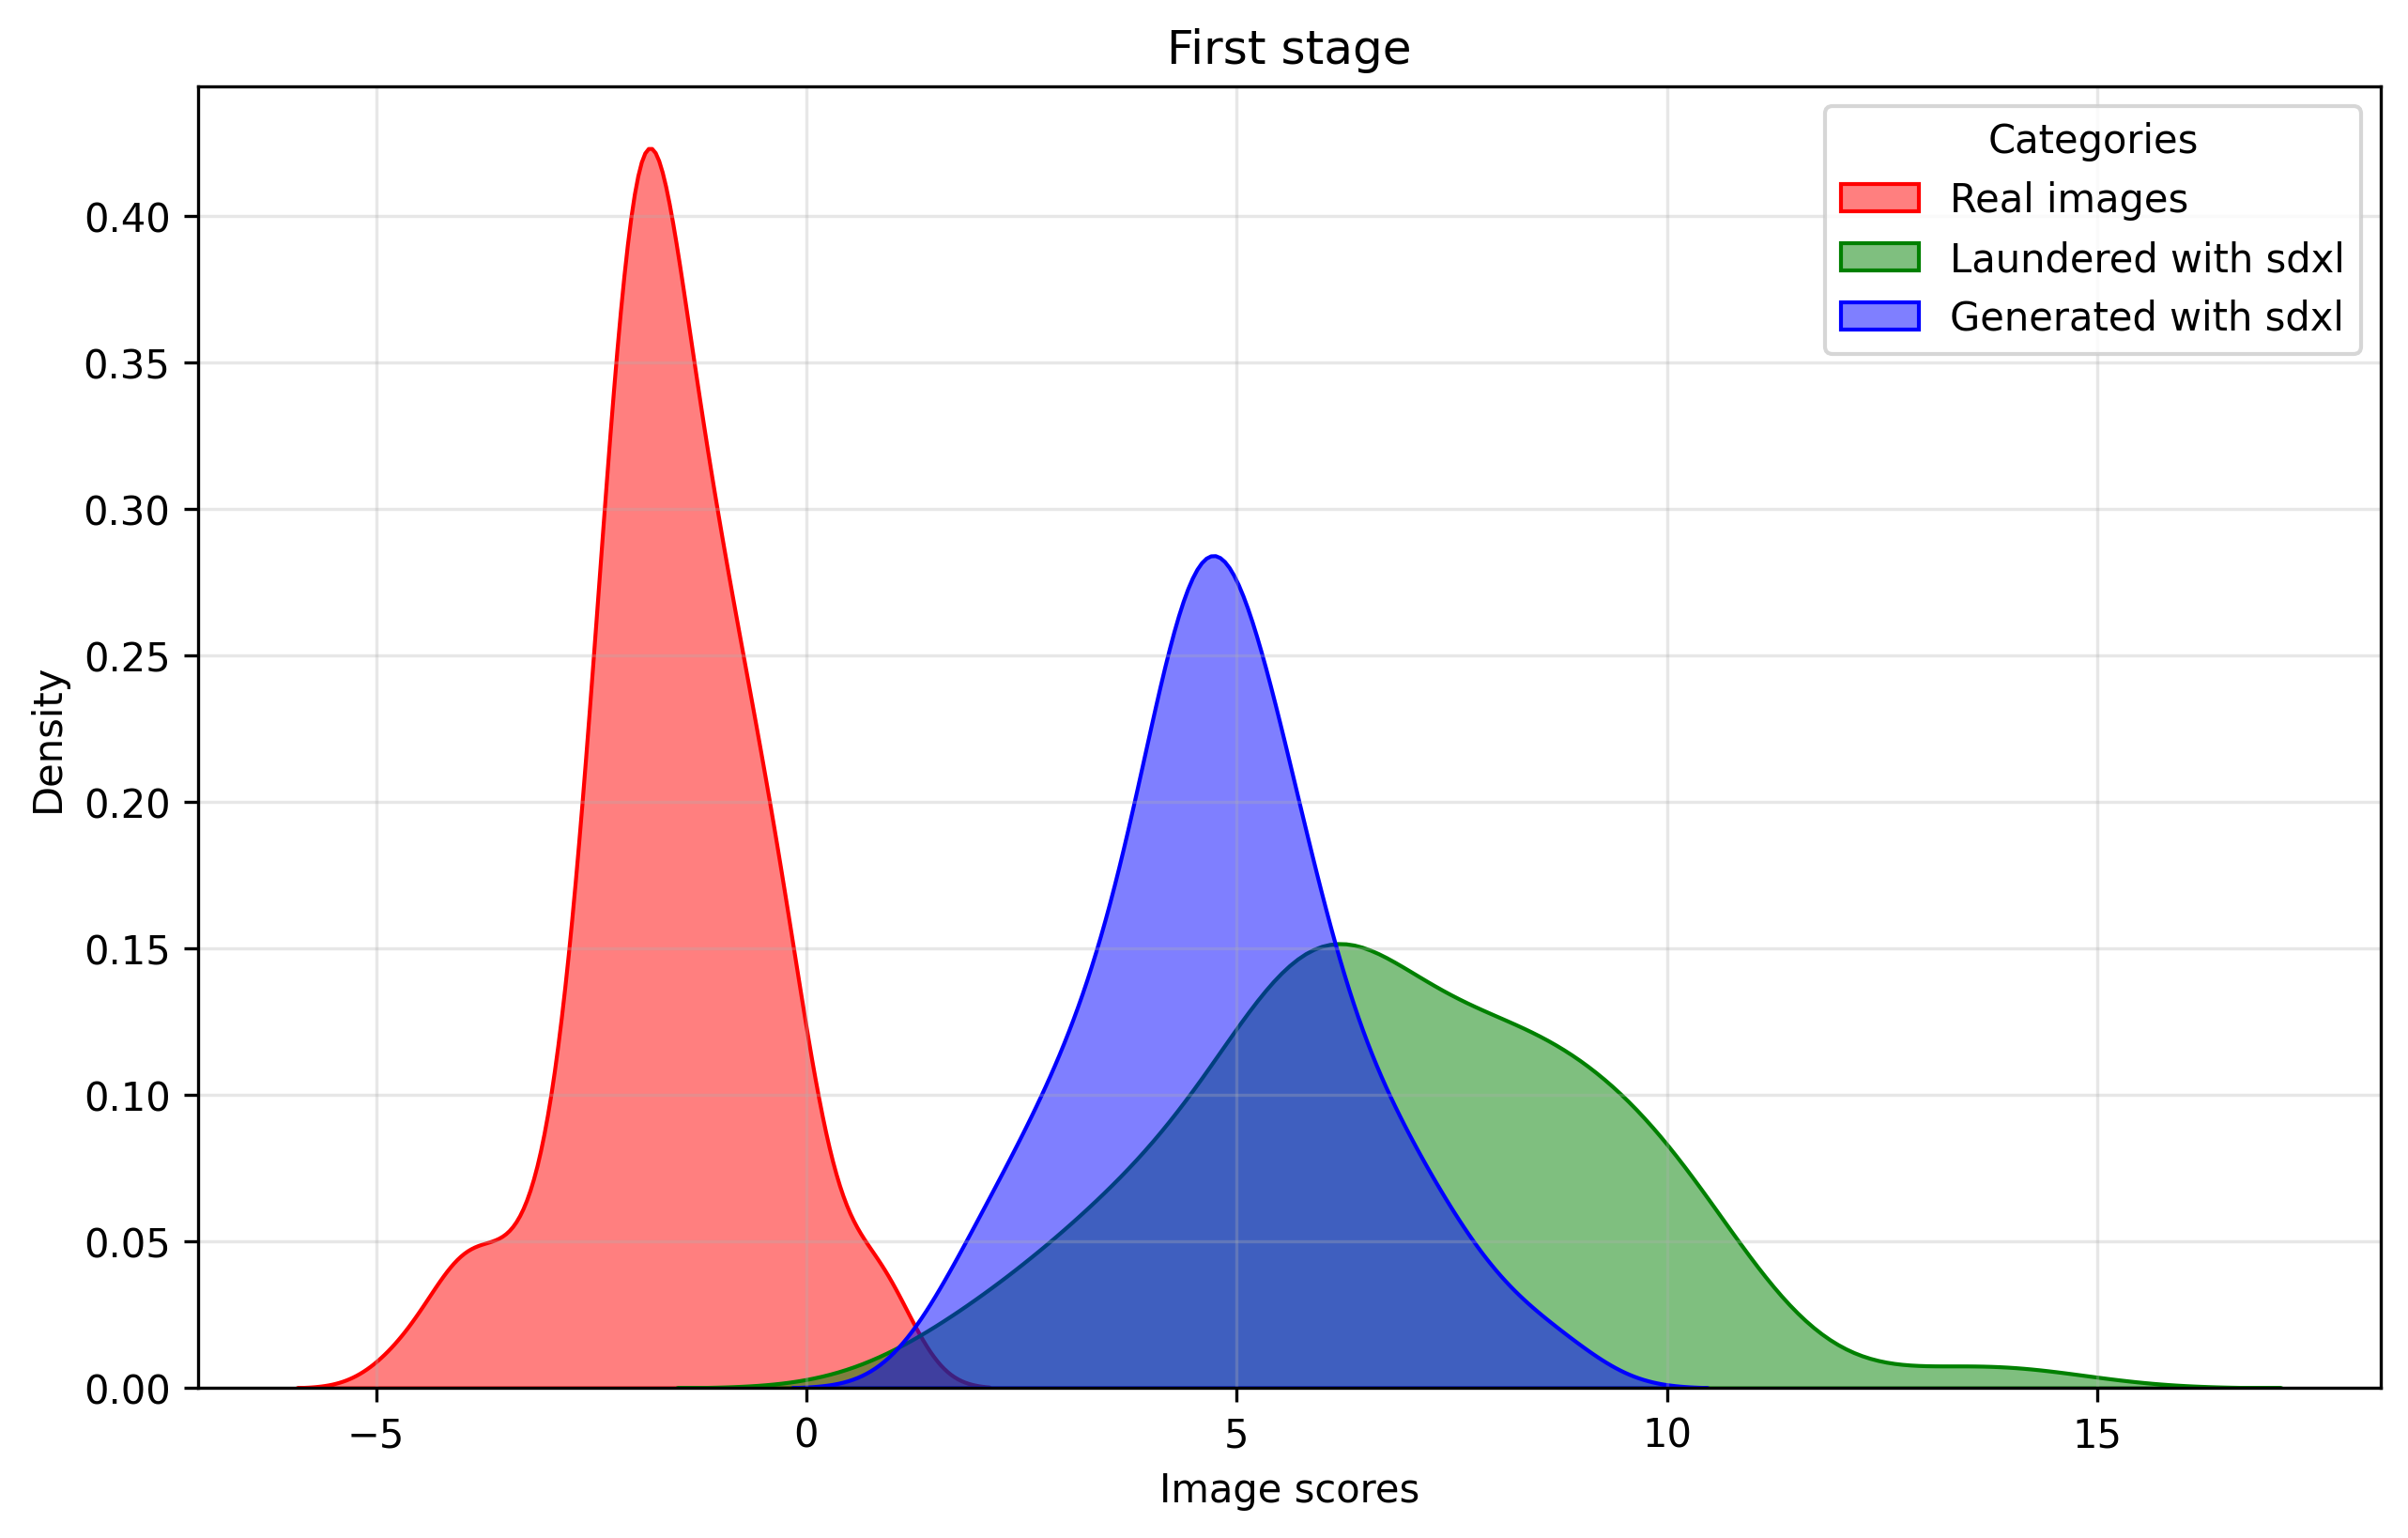
\includegraphics[width=0.8\linewidth]{Img/First_stage.png}
    %    \caption{Esempio di immagine.}
    %    \label{fig:esempio}
    %\end{figure}



    \subsection{PIZZA}
\section{Attacks}
    \subsection{Mimicry}
    \subsection{SD Laundering}
    \subsection{White Black}
    \subsection{Adversarial Robustness}
\section{Experiment}
\section{Conclusions}

\bibliographystyle{IEEEtran} % Stile delle referenze (es. IEEE)
\bibliography{references}    % Nome del file .bib (senza estensione)

\end{document}